
\title{Analisi dell'Errore}
\author{
        Sebastiano Caccaro
}


\documentclass[12pt]{article}
\usepackage[utf8]{inputenc}
\usepackage{amssymb}
\usepackage{amsmath}
\usepackage[italian]{babel}
\usepackage{hyperref}
\usepackage{color,soul}
\usepackage{float}
\usepackage{listings}
\usepackage{tikz}
\usetikzlibrary{positioning}


\lstset{  
  xleftmargin=0.05\textwidth, xrightmargin=.2\textwidth,
}

\begin{document}
\maketitle
\newcommand{\E}{È}


\abstract{In questo documento è presentata l'analisi dell'errore di sostituzione e la sua correggibilità con sistema di correzione basato sul mask-filling tramite modello BERT.}

\section{Analisi prestazioni BERT}
\subsection{Introduzione}
Il sistema di correzione sviluppato sfrutta la funzione di mask-filling dei modelli BERT. \\
In breve, una volta identificato un token non corretto, esso viene mascherato e il sistema propone una serie di proposte, ciascuna accompagnata dalla probabilità che la parola suggerita sia quella corretta.
Ad esempio, presa la frase:
\begin{center}
\textit{"celebrare la venuta dello \underline{Spiito} Santo, noi vi invitiamo ad implorare da Lui il dono della gioia."}
\end{center}
si può notare come il token sottolineato sia un errore. Esso viene quindi mascherato per ottenere la seguente frase:
\begin{center}
\textit{"celebrare la venuta dello [MASK] Santo, noi vi invitiamo ad implorare da Lui il dono della gioia."}
\end{center}
Il sistema propone quindi n candidati per questa la frase data in input, di seguito i primi 5:
\begin{itemize}
\item  \textit{"Spirito"} con probabilità 0.999
\item  \textit{"spirito"} con probabilità 7.78e-05
\item  \textit{"Spazio"} con probabilità 7.36e-06
\item  \textit{"stesso"} con probabilità 4.31e-06
\item  \textit{"Zo"} con probabilità 3.85e-06
\end{itemize}
Per correggere l'errore sono quindi necessarie due condizioni:
\begin{itemize}
\item Fra le parole fornite da BERT deve essere presente quella corretta
\item Se si verifica la prima condizione, è necessario scegliere la parola corretta
\end{itemize}
Dalla prima condizione si evince come le prestazioni di BERT siano un limite superiore per ogni sistema che ne usi l'output per effettuare correzioni. Trovando il limite superiore è quindi possibile analizzare in modo più accurato i sistemi di correzione implementati.

\subsection{Metodologia dell'analisi}
L'analisi dell'errore riguarda solo ed esclusivamente l'ambito della correzione. \E\ quindi necessario che i risultati finali non siano sporcati da altri fattori, come l'error detection.\\
A questo scopo è stato derivato un nuovo dataset a partire da quello usato per i test di correzione. Innanzitutto vengono estratte delle frasi a campione:
\begin{itemize}
\item 3500 per ciascun livello di perturbazione (T1, T2, T3, S1, S2, S3, M1, M2, M3)
\item 3500 non perturbate
\end{itemize}
per un totale di 35000 frasi.\\
In ognuna di queste frasi viene perturbato un solo token, e viene memorizzata la parola originale. Il token perturbato deve per forza essere presente all'interno di un vocabolario predeterminato, in modo da evitare che token già perturbati vengano ri-perturbati. Il token perturbato viene quindi memorizzato, così come la frase già mascherata. \E\ inoltre memorizzato anche il livello di perturbazione della frase originale.\\
Viene presentato in seguito un esempio del processo appena descritto.\\
La frase presa a campione
\begin{center}
\textit{"rarissima', di cui. il Signore si serve per venire a nostro contatto"}
\end{center}
viene mappata nel seguente set:

\begin{itemize}
\item Frase: \textit{"rarissima', di cui. il Signore [MASK] serve per venire a nostro contatto"} 
\item Token perturbato: ss
\item Token originale: si
\item Livello di perturbazione: M2
\end{itemize}

In questo modo sarà in seguito possibile riprodurre il processo di correzione e confrontare i risultati con la soluzione corretta.\\
Una volta ottenuto questo dataset, per ogni frase vengono trovati i candidati di correzione proposti da BERT, che vengono aggiunti aggiunti al precedente set insieme alla loro probabilità associata.

\subsection{Metriche}
L'analisi è mirata a fornire le seguenti statistiche:
\begin{itemize}
\item \textbf{Correzioni possibili:} percentuale delle volte in cui la correzione corretta è presente nei primi n risultati forniti da BERT. In questo modo è possibile trovare il limite superiore per ogni sistema di correzione che ne faccia uso.
\item \textbf{Distribuzione delle correzioni:} il ranking di ogni correzione corretta fra i risultati forniti da bert ordinati per probabilità.
\end{itemize}

\subsection{Risultati}
Per la misurazione delle correzioni possibili è stato scelto di misurare 3 diverse soglie: viene rilevata la presenza del correzione corretta nei primi 10, primi 20 e primi 30 risultati forniti da BERT.


\begin{figure}[H]
\centering
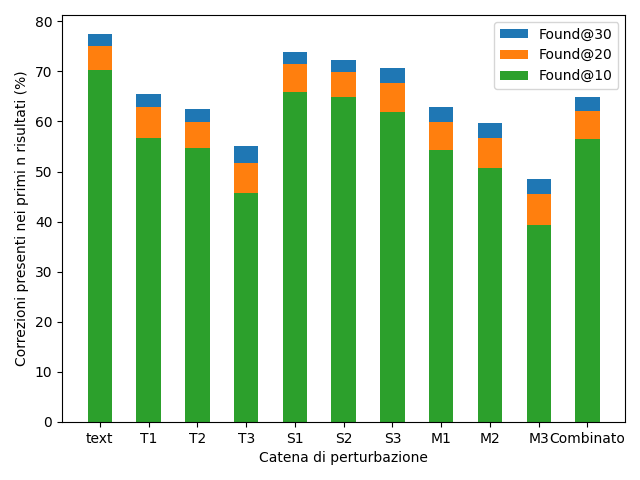
\includegraphics[width=\textwidth]{distributions/overview.png}
\caption{Correzioni presenti nei primi n risultati prodotti da BERT in percentuale}
\end{figure}


%\begin{figure}[H]
%\centering
%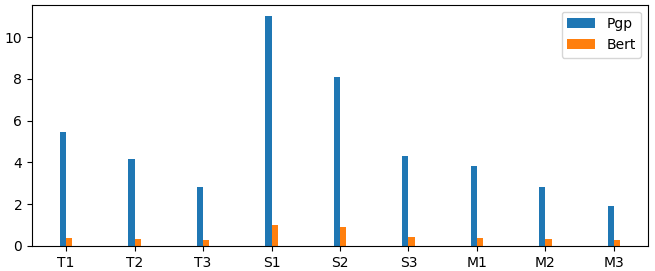
\includegraphics[width=\textwidth]{immagini/ipc}
%\caption{Rapporto fra gli errori erroneamente introdotti dal processo di correzione e gli errori corretti dallo stesso processo}
%\end{figure}


%\begin{table}[H]
%\centering
%\begin{tabular}{c|cc|cc|cc}
%& \multicolumn{2}{c}{\textbf{Metrica 1}} & \multicolumn{2}{c}{\textbf{Metrica 2}} & \multicolumn{2}{c}{\textbf{Metrica 3}} \\
%& Bert & Pgp & Bert & Pgp & Bert & Pgp \\ \hline
%T1 & 0.4 & 0.24 & 0.41 & 2.17 & 0.32 & 2.8 \\
%T2 & 0.4 & 0.27 & 0.42 & 2.15 & 0.26 & 1.96 \\
%T3 & 0.37 & 0.28 & 0.48 & 2.21 & 0.22 & 1.36 \\
%S1 & 0.27 & 0.15 & 0.36 & 2.0 & 0.91 & 9.38 \\
%S2 & 0.25 & 0.17 & 0.36 & 1.96 & 0.83 & 6.4 \\
%S3 & 0.28 & 0.16 & 0.39 & 1.8 & 0.44 & 3.53 \\
%M1 & 0.32 & 0.22 & 0.47 & 2.08 & 0.35 & 2.3 \\
%M2 & 0.33 & 0.25 & 0.47 & 2.0 & 0.26 & 1.49 \\
%M3 & 0.26 & 0.24 & 0.65 & 2.04 & 0.3 & 1.05 \\
%\end{tabular}
%\caption{Risultati sperimentali del correttore BERT e del correttore Pgp con frasi di lunghezza 100}
%\end{table}















\end{document}